\chapter{Nuevo Sistema de Entrenamiento}\label{chap:2}
En este capítulo se presentará la propuesta de solución para este nuevo sistema de entrenamiento que se desea conseguir. Para que el desarrollo de un proyecto concluya con éxitos, primero debe realizarse un diseño completo de lo que se pretende obtener, así como los recursos y requisitos que debe poseer. A lo largo del capítulo se tratarán de presentar numerosos diagramas para facilitar la comprensión. Cabe destacar que este nuevo diseño parte del SECPROIT, por lo que se realizarán algunas comparaciones con ese sistema.

\section{Modelado del Negocio}
Los modelos se crean con el objetivo de entender mejor la entidad real que se va a construir. Deben cumplir con objetivos diferentes, niveles de abstracción, con la ilustración del software desde el punto de vista del cliente y después con su representación en un nivel más técnico.

\subsection{Modelo de Dominio}
El modelo de dominio es una representación de las clases conceptuales del mundo real, no de componentes de software. Se muestran los conceptos significativos en un dominio del problema. Para una mejor comprensión del modelo, es necesario entender las entidades que influyen en el negocio.

En la Figura \ref{fig:modelD}, se puede apreciar el modelo de dominio para este nuevo sistema. Es muy semejante, en cuanto a lógica del negocio, al modelo del SECPROT.

Las áreas de color verde, indica que se ha modificado la entidad para ajustarla a los nuevos cambios que se decidieron hacer. Los cambios más significativos son aquellas entidades que se modificaron casi en su totalidad o aquellas que fueron agregadas de cero. Estas últimas están representadas con un color amarillo. 

\begin{figure}[h]
\centering
 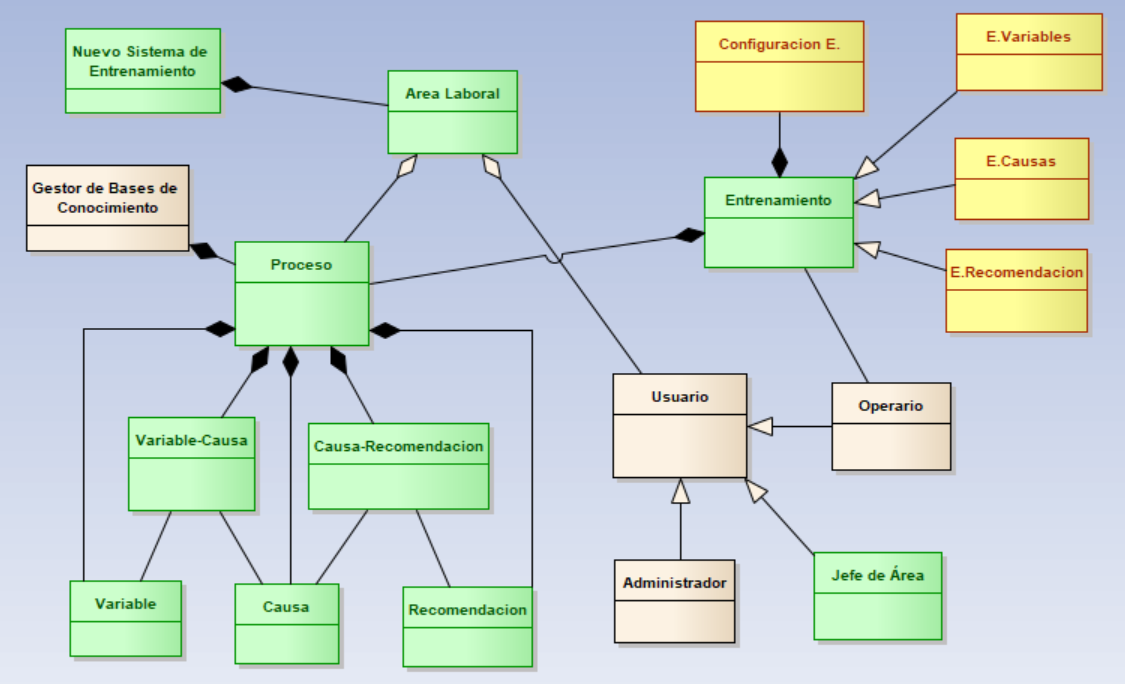
\includegraphics[width=0.5\linewidth]{imagen/dominio.png}
 \caption{Modelo de Dominio del Nuevo Sistema.}
 \label{fig:modelD} 
\end{figure} 

Como bien se aprecia, el diagrama indica que se han creado cuatro nuevas entidades: configuración de entrenamiento, entrenamiento de variables, entrenamiento de causas y entrenamiento de recomendaciones. Estas entidades fueron creadas para un mejor manejo de la información de la capacitación, y para introducir una nueva regla: separar los entrenamientos por etapas.

\subsection{Reglas del Negocio}
Cada negocio posee un conjunto de restricciones que permiten su correcto funcionamiento. Estas restricciones son conocidas como reglas del negocio.
Las reglas a cumplir en este nuevo sistemas son:

\begin{itemize}
\item Antes de crear un usuario, deben haberse creado los roles del sistema y las áreas laborales.
\item Antes de crear un proceso, deben haberse creado las áreas laborales.
\item Antes de crear un entrenamiento debe existir un proceso y al menos un operario.
\item Antes de realizar el entrenamiento de las causas se debe haber aprobado el entrenamiento de las variables.
\item Antes de realizar el entrenamiento de las recomendaciones se debe haber aprobado el entrenamiento de las causas.
\item Los usuarios solo pueden poseer un rol.
\item Los usuarios solo pueden pertenecer a un área a la vez.
\item Los procesos solo pueden pertenecer a un área a la vez.
\item Las tareas de los roles son únicas para el usuario, es decir, solo las pueden hacer los usuarios con el mismo rol.
\end{itemize} 

\subsection{Diagrama de Actividades}
Un diagrama de actividades recoge una vista dinámica de alto nivel, del flujo principal del proceso. En el mismo, se tienen en cuenta las entidades que participan en el negocio y las acciones que realizan cada una, así como los llamados objetos con los que se trabaja. En estos diagramas se representa el inicio y el fin del flujo.

En esta propuesta de solución, el flujo del administrador resulta el mismo que el del sistema SECPROIT \cite{elena}. Sin embargo, el flujo de los operarios y jefes de área cambia. En la Figura \ref{fig:actividades}, se representa el diagrama de actividades de estos dos roles, detallando el nuevo flujo de los mismos.

\begin{figure}[h]
\centering
 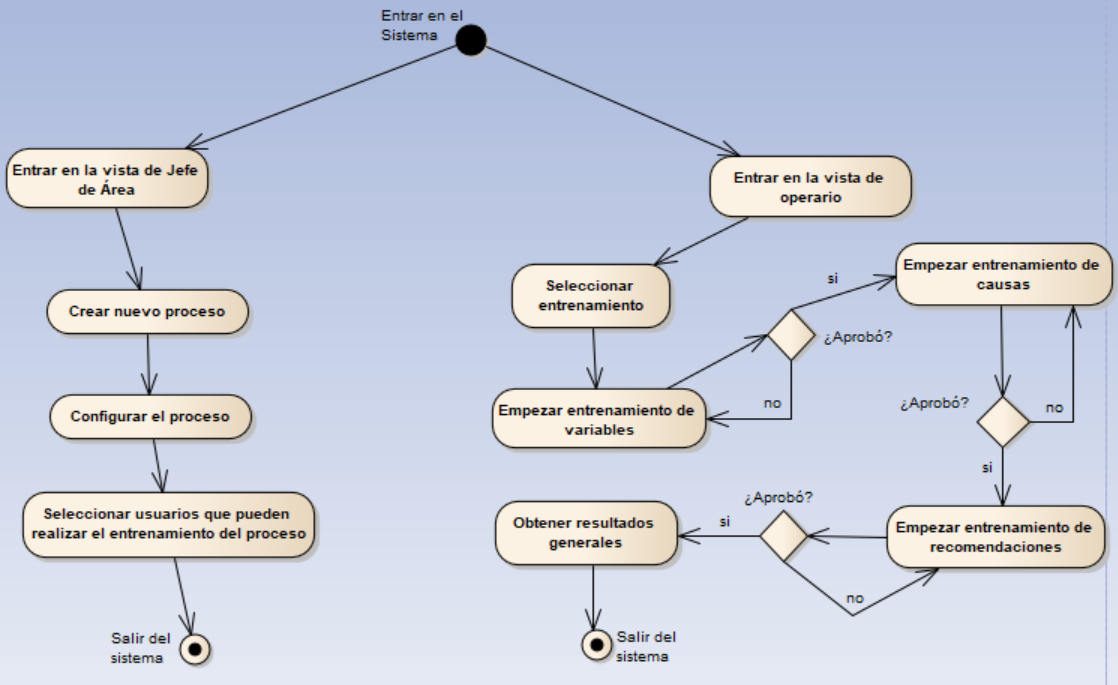
\includegraphics[width=0.5\linewidth]{imagen/actividades.png}
 \caption{Diagrama de Actividades del Nuevo Sistema.}
 \label{fig:actividades} 
\end{figure} 